% tikz_codes.tex -- twenty-four-point codes at positive slack (Proposition 2.28, Remark 2.29).
%   (a) The inner products of the 276 pairs: the root system (96 at 1/2, 72 at 0, 96 at -1/2,
%       12 at -1) against the second code of Proposition 2.28 (largest inner product 0.516978).
%   (b) The deepest hole of a 24-point code of slack s: the least value of max_i <theta, w_i>
%       found over codes of slack s and directions theta (floating point, local optimisation).
%       A further centre within sqrt6 beside 24 centres within 2.0161 needs 0.6141 or less.
%   (c) The least contact-cell volume found over 24-point codes of slack s: the root system and
%       the curves of Proposition 2.26 give 8; codes away from the root system give the open marks.
% Build:  pdflatex tikz_codes.tex && pdftoppm -r 500 -png -singlefile tikz_codes.pdf ../figures/fig_tikz_codes
% Test:   python3 tikz_overlap_check.py --auto tikz_codes.tex
\documentclass[border=4pt]{standalone}
\usepackage{tikz}
\usepackage{pgfplots}
\pgfplotsset{compat=1.17}
\usetikzlibrary{positioning,arrows.meta,calc}
\usepackage[T1]{fontenc}
\usepackage{lmodern}
\usepackage{amsmath,amssymb}
\definecolor{cblue}{HTML}{2A78D6}
\definecolor{corange}{HTML}{EB6834}
\definecolor{caqua}{HTML}{1BAF7A}
\definecolor{cviolet}{HTML}{7A5AC8}
\definecolor{cink2}{HTML}{52514E}
\definecolor{cink3}{HTML}{8B8A85}
% tikzcheck.tex -- the hooks of tikz_overlap_check.py, input by the TikZ figures.
% Two ways to name what is checked.
%  - Explicit: \figboxes and \figlabels list named nodes; with \nolabels defined,
%    nodes in the style lbl are drawn invisibly.
%  - Automatic: \autocheck in the preamble gives every node of the picture,
%    pgfplots tick labels included, an alias chk<n>; with \nolabels defined, the
%    text of every node is drawn invisibly and its shape is kept.
% \checkfigure, at the end of the picture, writes the four corners of each
% checked node (so that rotated nodes are measured by their true extent) and
% those of the picture to the log when \checkbboxes is defined.
\tikzset{lbl/.style={}}
\ifdefined\nolabels\tikzset{lbl/.append style={opacity=0}}\fi
\newcount\chknodes
\newcommand\autocheck{% idempotent: a figure with \autocheck may also be run with --auto
  \ifdefined\chkauto\else
  \def\chkauto{}%
  \tikzset{every node/.append style={/utils/exec={\global\advance\chknodes by 1\relax},
                                      alias=chk\the\chknodes}}%
  \ifdefined\nolabels\tikzset{every node/.append style={text opacity=0}}\fi
  \fi}
\makeatletter
% a node counted but never kept (pgfplots typesets some nodes once to measure them)
% has no shape, and is skipped
\newcommand\chkifnode[2]{\pgfutil@ifundefined{pgf@sh@ns@#1}{}{#2}}
\makeatother
\newcommand\chkout[2]{% kind, node
  \path let \p1=(#2.south west), \p2=(#2.north east), \p3=(#2.north west), \p4=(#2.south east)
    in \pgfextra{\typeout{BBOX #1 #2\space\x1\space\y1\space\x2\space\y2\space\x3\space\y3\space\x4\space\y4}};}
\newcommand\checkfigure{%
  \ifdefined\checkbboxes
    \path let \p1=(current bounding box.south west), \p2=(current bounding box.north east)
      in \pgfextra{\typeout{PICBB \x1\space\y1\space\x2\space\y2}};
    \typeout{BORDER 4.0pt}%
    \ifdefined\chkauto
      \edef\chklast{\the\chknodes}%
      \foreach \nm in {1,...,\chklast} {\chkifnode{chk\nm}{\chkout{auto}{chk\nm}}}%
    \else
      \foreach \nm in \figboxes {\chkout{box}{\nm}}%
      \foreach \nm in \figlabels {\chkout{label}{\nm}}%
    \fi
  \fi}
\ifdefined\forceauto\autocheck\fi

\autocheck
\begin{document}
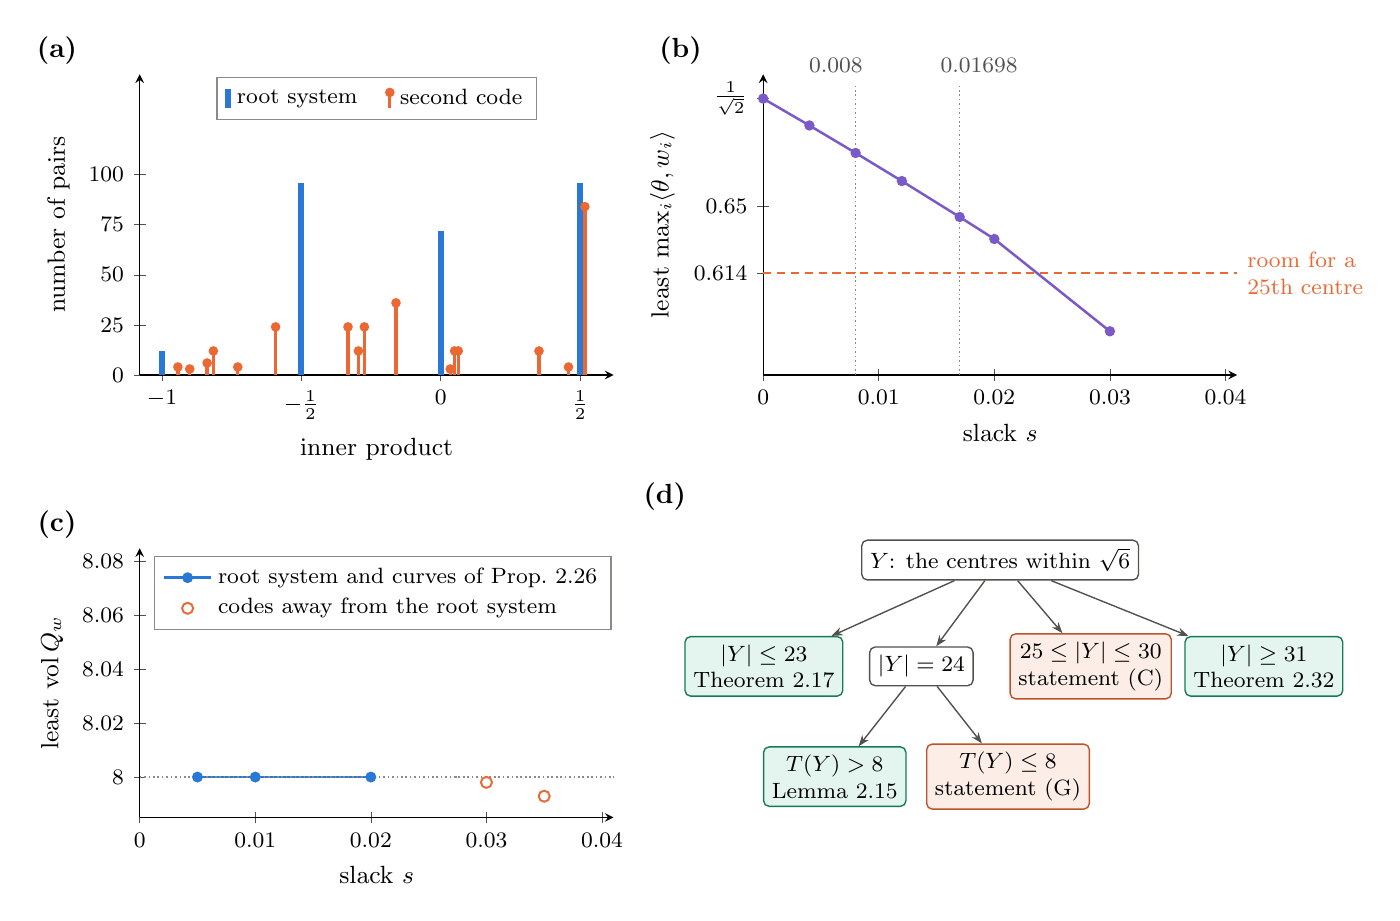
\begin{tikzpicture}[font=\small]
%% (a) spectra
\begin{axis}[name=A, width=7.6cm, height=5.4cm, xmin=-1.08, xmax=0.62, ymin=0, ymax=150,
    xtick={-1,-0.5,0,0.5}, xticklabels={$-1$,$-\tfrac12$,$0$,$\tfrac12$},
    ytick={0,25,50,75,100},
    xlabel={inner product}, ylabel={number of pairs},
    axis lines=left, tick style={cink2}, tick label style={font=\footnotesize},
    legend cell align=left, legend columns=2, legend style={font=\footnotesize, at={(0.5,0.99)}, anchor=north, draw=cink3, fill=white, /tikz/every even column/.append style={column sep=8pt}},
    clip=false]
  \addplot[ycomb, cblue, line width=2.2pt, legend image code/.code={\draw[cblue, line width=2.2pt] (0.15cm,-0.12cm) -- (0.15cm,0.12cm);}] coordinates {(-1,12) (-0.5,96) (0,72) (0.5,96)};
  \addlegendentry{root system}
  \addplot[ycomb, corange, line width=1.2pt, mark=*, mark size=1.1pt, legend image code/.code={\draw[corange, line width=1.2pt] (0.15cm,-0.12cm) -- (0.15cm,0.08cm); \fill[corange] (0.15cm,0.08cm) circle (1.1pt);}] coordinates {
    (0.5170,84) (0.4583,4) (0.3524,12) (0.0628,12) (0.0498,12) (0.0340,3)
    (-0.1605,36) (-0.2740,24) (-0.2953,12) (-0.3327,24) (-0.5924,24) (-0.7282,4)
    (-0.8157,12) (-0.8380,6) (-0.9004,3) (-0.9429,4)};
  \addlegendentry{second code}
\end{axis}
\node[font=\bfseries] at ($(A.north west)+(-1.05cm,0.3cm)$) {(a)};
%% (b) deepest hole
\begin{axis}[name=B, at={($(A.east)+(1.9cm,0)$)}, anchor=west, width=7.6cm, height=5.4cm,
    xmin=0, xmax=0.041, ymin=0.56, ymax=0.72,
    xtick={0,0.01,0.02,0.03,0.04}, xticklabels={$0$,$0.01$,$0.02$,$0.03$,$0.04$}, scaled x ticks=false, ytick={0.6141,0.65,0.7071},
    yticklabels={$0.614$,$0.65$,$\tfrac1{\sqrt2}$},
    xticklabel style={/pgf/number format/fixed},
    xlabel={slack $s$}, ylabel={least $\max_i\langle\theta,w_i\rangle$},
    axis lines=left, tick style={cink2}, tick label style={font=\footnotesize},
    clip=false]
  \addplot[cviolet, line width=0.9pt, mark=*, mark size=1.4pt] coordinates {
    (0,0.70711) (0.004,0.69280) (0.008,0.67817) (0.012,0.66322) (0.017,0.64409) (0.020,0.63238) (0.030,0.58327)};
  \addplot[corange, densely dashed, line width=0.7pt, domain=0:0.041] {0.6141};
  \draw[cink3, densely dotted, line width=0.6pt] (axis cs:0.008,0.56) -- (axis cs:0.008,0.715);
  \draw[cink3, densely dotted, line width=0.6pt] (axis cs:0.01698,0.56) -- (axis cs:0.01698,0.715);
  \coordinate (Bk) at (axis cs:0.008,0.715);
  \coordinate (Bs) at (axis cs:0.01698,0.715);
  \coordinate (Bl) at (axis cs:0.0405,0.6141);
\end{axis}
\node[font=\footnotesize, text=cink2, anchor=south] at ($(Bk)+(-0.25,0.02)$) {$0.008$};
\node[font=\footnotesize, text=cink2, anchor=south] at ($(Bs)+(0.25,0.02)$) {$0.01698$};
\node[font=\footnotesize, text=corange, anchor=west, align=left] at ($(Bl)+(0.08,0)$) {room for a\\ $25$th centre};
\node[font=\bfseries] at ($(B.north west)+(-1.05cm,0.3cm)$) {(b)};
%% (c) contact cells
\begin{axis}[name=Cc, at={($(A.south)+(0,-2.2cm)$)}, anchor=north, width=7.6cm, height=5.0cm,
    xmin=0, xmax=0.041, ymin=7.985, ymax=8.085,
    xtick={0,0.01,0.02,0.03,0.04}, xticklabels={$0$,$0.01$,$0.02$,$0.03$,$0.04$}, scaled x ticks=false, ytick={8,8.02,8.04,8.06,8.08},
    xticklabel style={/pgf/number format/fixed},
    yticklabel style={/pgf/number format/fixed, /pgf/number format/precision=2},
    xlabel={slack $s$}, ylabel={least $\operatorname{vol}Q_w$},
    axis lines=left, tick style={cink2}, tick label style={font=\footnotesize},
    legend cell align=left, legend style={font=\footnotesize, at={(0.03,0.97)}, anchor=north west, draw=cink3, fill=white},
    clip=false]
  \addplot[cblue, line width=0.9pt, mark=*, mark size=1.5pt] coordinates {(0.005,8) (0.010,8) (0.020,8)};
  \addlegendentry{root system and curves of Prop.~2.26}
  \addplot[only marks, corange, mark=o, mark size=2pt, line width=0.7pt] coordinates {(0.020,8.06791) (0.030,7.99802) (0.035,7.99288)};
  \addlegendentry{codes away from the root system}
  \addplot[cink3, densely dotted, line width=0.6pt, domain=0:0.041] {8};
\end{axis}
\node[font=\bfseries] at ($(Cc.north west)+(-1.05cm,0.3cm)$) {(c)};
%% (d) the reduction of Proposition 2.30, as a schematic
\begin{scope}[shift={($(B.south)+(0,-2.35cm)$)}, font=\footnotesize,
    box/.style={draw=cink2, rounded corners=2pt, fill=white, align=center, inner sep=3pt, line width=0.5pt},
    ok/.style={box, fill=caqua!12, draw=caqua!70!black},
    open/.style={box, fill=corange!12, draw=corange!80!black},
    arr/.style={-{Stealth[length=4pt]}, cink2, line width=0.5pt}]
  \node[box] (Y) at (0,0) {$Y$: the centres within $\sqrt6$};
  \node[ok] (m23) at (-3.0,-1.35) {$|Y|\le23$\\ Theorem 2.17};
  \node[box] (m24) at (-1.0,-1.35) {$|Y|=24$};
  \node[open] (m25) at (1.15,-1.35) {$25\le|Y|\le30$\\ statement (C)};
  \node[ok] (m31) at (3.35,-1.35) {$|Y|\ge31$\\ Theorem 2.32};
  \node[ok] (T8) at (-2.1,-2.75) {$T(Y)>8$\\ Lemma 2.15};
  \node[open] (G) at (0.1,-2.75) {$T(Y)\le8$\\ statement (G)};
  \draw[arr] (Y) -- (m23);
  \draw[arr] (Y) -- (m24);
  \draw[arr] (Y) -- (m25);
  \draw[arr] (Y) -- (m31);
  \draw[arr] (m24) -- (T8);
  \draw[arr] (m24) -- (G);
\end{scope}
\node[font=\bfseries] at ($(B.south west)+(-1.25cm,-1.55cm)$) {(d)};
\checkfigure
\end{tikzpicture}
\end{document}
